\documentclass[12pt,addpoints]{evalua}
\grado{2$^\circ$ de Secundaria}
\cicloescolar{2024-2025}
\materia{Matemáticas 2}
\unidad{1}
\title{Examen de la Unidad}
\aprendizajes{%
      \item Resuelve problemas de multiplicación y división con números enteros, fracciones y decimales positivos y negativos.
      \item Resuelve problemas de potencias con exponente entero y aproxima raíces cuadradas.
      \item Resuelve problemas que impliquen el uso de la notación científica.
      \item Calcula porcentajes de cantidades.
}
\author{Prof.: Julio César Melchor Pinto}
\begin{document}%
\begin{multicols}{2}
	\tableofcontents
\end{multicols}\newpage
\begin{questions}\large
	\addcontentsline{toc}{section}{Cálculos numéricos}
	\section*{Cálculos numéricos}

      \question[10] Realiza las siguientes operaciones de \textit{cálculo numérico}:
   
      \begin{parts}
            \begin{multicols}{2}
                  
\addcontentsline{toc}{subsection}{Suma de números}
	\subsection*{Suma de números}

                  \part $899.882+242.2+469.381=$ \fillin[$1611.463$][0in]
                  % \part \ifprintanswers{\opmanyadd[style=text]{899.882}{242.2}{469.381}}
			% 	\else{\opmanyadd[style=text,resultstyle=\color{white}]{849.882}{242.2}{469.381}}\fi

                        \addcontentsline{toc}{subsection}{Resta de números}
	\subsection*{Resta de números}

                  \part $4934-451-682=$ \fillin[$3801$][0in]
                  % \part
			% 	\ifprintanswers{\opmanysub[hfactor=decimal,resultstyle=\color{red},carrysub=true,style=text]{4934}{451}{682}}
			% 	\else{\opmanysub[hfactor=decimal,resultstyle=\color{white},carrysub=false,style=text]{4934}{451}{682}}\fi\\[0.2cm]

                        \addcontentsline{toc}{subsection}{Multiplicación de números}
	\subsection*{Multiplicación de números}

                  % \part $19.8\times6.27=$ \fillin[$121.011$][0in]
                  \part \ifprintanswers{\opmul[hfactor=decimal,style=text,resultstyle=\color{red},displayintermediary=None]{19.3}{6.27}}
                  \else{$19.8\times6.27=$}\fi

\addcontentsline{toc}{subsection}{División de números}
	\subsection*{División de números}

                  % \part $924\divisionsymbol1.1=$ \fillin[$840$][0in]
                  \part \ifprintanswers{\opdiv[hfactor=decimal,style=text,resultstyle=\color{red}]{924}{1.1}}
                  \else{$924\divisionsymbol1.1=$}\fi

            \end{multicols}
            
\addcontentsline{toc}{subsection}{Resolución de problemas}
	\subsection*{Resolución de problemas}

            \part Entre José y su hermano están arreglando el jardín de su casa. José arregló $\dfrac{3}{8}$ del jardín y su hermano $\dfrac{1}{4}$. ¿Qué parte del jardín han arreglado?
           
            \begin{solutionbox}{1.8cm}
                  \[\dfrac{1}{8}+\dfrac{3}{4}=\dfrac{1}{8}+\dfrac{6}{8}=\dfrac{7}{8}\]
            \end{solutionbox}
      \end{parts}

      % \newpage

      \addcontentsline{toc}{section}{Números negativos}
	\section*{Números negativos}

      
\addcontentsline{toc}{subsection}{Ubicación en la recta numérica}
	\subsection*{Ubicación en la recta numérica}

      \question[4] Escribe el número que representa el punto indicado en la recta numérica de cada uno de los siguientes incisos.

      \begin{multicols}{2}
            \begin{parts}
                  \part 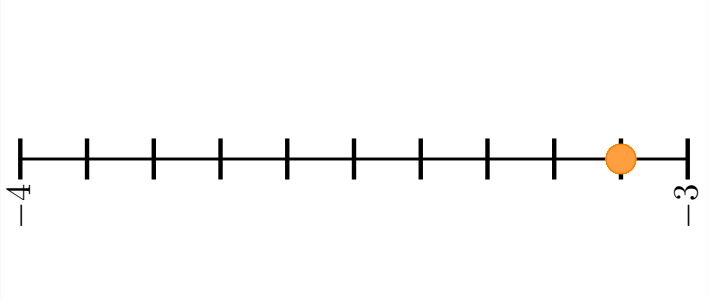
\includegraphics[width=180px]{../images/recta_num_-3.1.png} \fillin[$-3.1$][1.5in]
                  \part 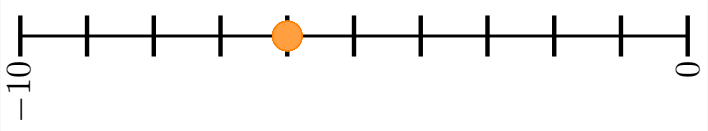
\includegraphics[width=180px]{../images/recta_num_-6.png}   \fillin[$-6$][1.5in]
                  \part 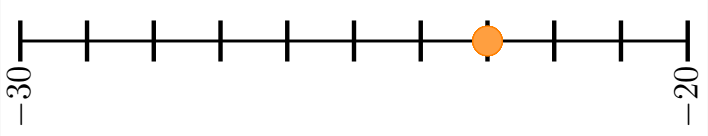
\includegraphics[width=180px]{../images/recta_num_-23.png}  \fillin[$-23$][1.5in]
                  \part 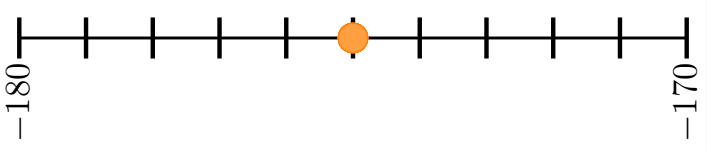
\includegraphics[width=180px]{../images/recta_num_-175.png} \fillin[$-175$][1.5in]

            \end{parts}
      \end{multicols}

      
\addcontentsline{toc}{subsection}{Comparación de negativos}
	\subsection*{Comparación de negativos}

      \question[6] Escribe sobre la línea el símbolo de mayor que ($>$), menor que ($<$), o igual ($=$) según corresponda.

      \begin{multicols}{2}
            \begin{parts}
                  \part $-51$  \fillin[$>$][0.3in] $-55$%\\[0.25em]
                  \part $-100$ \fillin[$<$][0.3in] $-99$%\\[0.25em]
                  \part $-182$ \fillin[$>$][0.3in] $-189$
                  \part $-36$  \fillin[$<$][0.3in] $-35$%\\[0.25em]
                  \part $-3.5$ \fillin[$<$][0.3in] $-2.2$%\\[0.25em]
                  \part $-97$  \fillin[$<$][0.3in] $-96.2$
            \end{parts}
      \end{multicols}

      \newpage
\addcontentsline{toc}{subsection}{Suma y resta con negativos}
	\subsection*{Suma y resta con negativos}

      \question[4] Realiza las siguientes sumas y restas con números negativos:

      \begin{multicols}{2}
            \begin{parts}
                  \part $-229+57=$ \fillin[$-172$][0in]
                  \part $198-189=$ \fillin[$9$][0in]
                  \part $-201.1-9.4=$ \fillin[$-210.5$][0in]
                  \part $(-15)-(-14)=$ \fillin[$-1$][0in]
            \end{parts}
      \end{multicols}

      
\addcontentsline{toc}{subsection}{Multiplicación y división con negativos}
	\subsection*{Multiplicación y división con negativos}

      \question[4] Realiza las siguientes multiplicaciones y divisiones con números negativos:
    
      \begin{multicols}{2}
            \begin{parts}
                                    \part $(-15)(-14)=$ \fillin[$210$][0in]
\part $(31)\divisionsymbol (-62)=$ \fillin[$-\dfrac{1}{2}$][0in]
\part $(0.25)(-50)=$ \fillin[$-12.5$][0in]
\part $(-220)\divisionsymbol (0.2)=$ \fillin[$-1100$][0in]

            \end{parts}
      \end{multicols}

      
\addcontentsline{toc}{subsection}{Potencias con números negativos}
	\subsection*{Potencias con números negativos}

      \question[4] Realiza las siguientes potencias de números negativos:
     
      \begin{multicols}{2}
            \begin{parts}
                  \part $-7^2=$ \fillin[$-49$][0in]
                  \part $-(-2)^4=$ \fillin[$-16$][0in]
                  \part $(-3)^3=$ \fillin[$-27$][0in]
                  \part $-(-5)^3=$ \fillin[$125$][0in]
            \end{parts}
      \end{multicols}


      \addcontentsline{toc}{section}{Exponentes y notación científica}
	\section*{Exponentes y notación científica}

      \question[6] Realiza las siguientes operaciones con exponentes:
   
      \begin{multicols}{3}
            \begin{parts}
                  
\addcontentsline{toc}{subsection}{Suma de exponentes}
	\subsection*{Suma de exponentes}

                  \part $(-5a^4)(-3a^2)=$ \fillin[$15a^6$][0in]
                  
\addcontentsline{toc}{subsection}{Resta de exponentes}
	\subsection*{Resta de exponentes}

                  \part $\dfrac{x^{13}y^{18}z^{4}}{x^{11}y^{9}z^{4}}=$ \fillin[$x^2y^9$][0in]
                  
\addcontentsline{toc}{subsection}{Multiplicación de exponentes}
	\subsection*{Multiplicación de exponentes}

                  \part $(a^3b^2c^4)^3=$ \fillin[$a^9b^6c^{12}$][0in]
            \end{parts}
      \end{multicols}

      % \newpage
      
\addcontentsline{toc}{subsection}{Notación científica}
	\subsection*{Notación científica}

      \question[4] Escribe en notación científica los siguientes números:
     
      \begin{multicols}{2}
            \begin{parts}
                  \part $0.00005=$ \fillin[$ 5\times10^{-5}$][0in]
                  \part $92000=$ \fillin[$ 9.2\times10^4$][0in]            
                  \part $0.00000000024=$ \fillin[$2.4 \cdot 10^{-10}$][0in]
                  \part $80008000=$ \fillin[$8.0008 \cdot 10^7$][0in]
            \end{parts}
            \end{multicols}
     
      \question[4] Escribe en notación decimal los siguientes números:
   
      \begin{multicols}{2}
            \begin{parts}
                  \part $6.7 \times 10^{4}=$ \fillin[$67000$][0in]
                  \part $7.2 \times 10^{-6}=$ \fillin[$0.0000072$][0in]            
                  \part $3.03 \cdot 10^{-3}=$ \fillin[$0.00303$][0in]
                  \part $3.1 \cdot 10^{6}=$ \fillin[$3100000$][0in]
            \end{parts}
      \end{multicols}

      \newpage
      \addcontentsline{toc}{section}{Plano cartesiano y la recta}
	\section*{Plano cartesiano y la recta}

      
\addcontentsline{toc}{subsection}{Ubicación en el plano cartesiano}
	\subsection*{Ubicación en el plano cartesiano}

      \question[10] Escribe las coordenadas de los puntos indicados en el plano cartesiano de cada uno de los siguientes incisos.
  
      \begin{multicols}{2}
            \begin{parts}
                  \part Coordenadas del punto A = \fillin[$(1,5)$][0in]
                  \part Coordenadas del punto B = \fillin[$(-3,6)$][0in]
                  \part Coordenadas del punto C = \fillin[$(5,-3)$][0in]
                  \part Coordenadas del punto D = \fillin[$(-5,0)$][0in]
                  \part Coordenadas del punto E = \fillin[$(0,-7)$][0in]
           
                  \addcontentsline{toc}{subsection}{Cuadrantes en el plano cartesiano}
	\subsection*{Cuadrantes en el plano cartesiano}
      
      \part Escribe el número del cuadrante en el que se encuentra el punto B en el plano cartesiano: \fillin[2 cuad.][1in]
      \end{parts}
            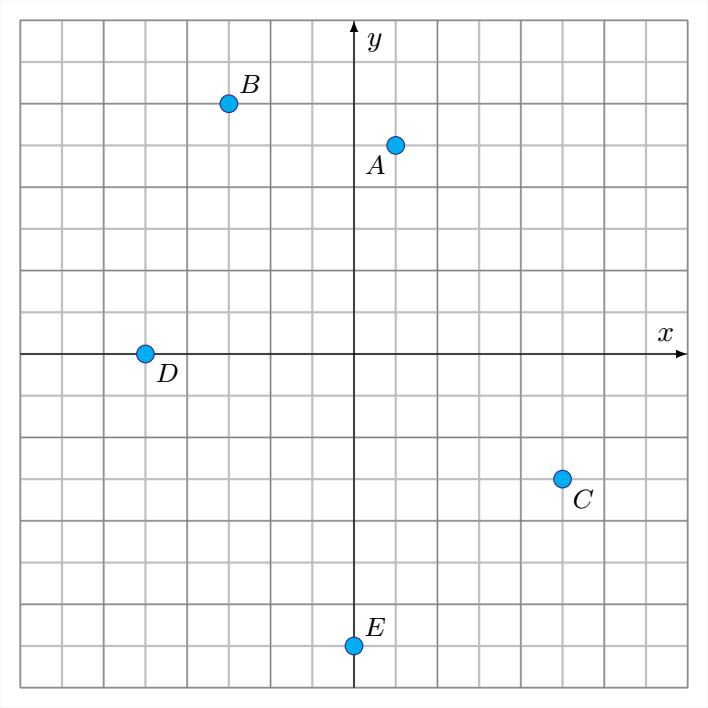
\includegraphics[width=0.8\linewidth]{../images/imagen_plano01.png}
      \end{multicols}

      



      % \newpage
      
\addcontentsline{toc}{subsection}{Pendiente de una recta}
	\subsection*{Pendiente de una recta}

      \question[8] Selecciona la opcion que corresponde a la pendiente de la recta en cada uno de los siguientes incisos:
    
      \begin{multicols}{2}
            \begin{parts}
                  \part
                  \begin{minipage}{0.5\linewidth}
                        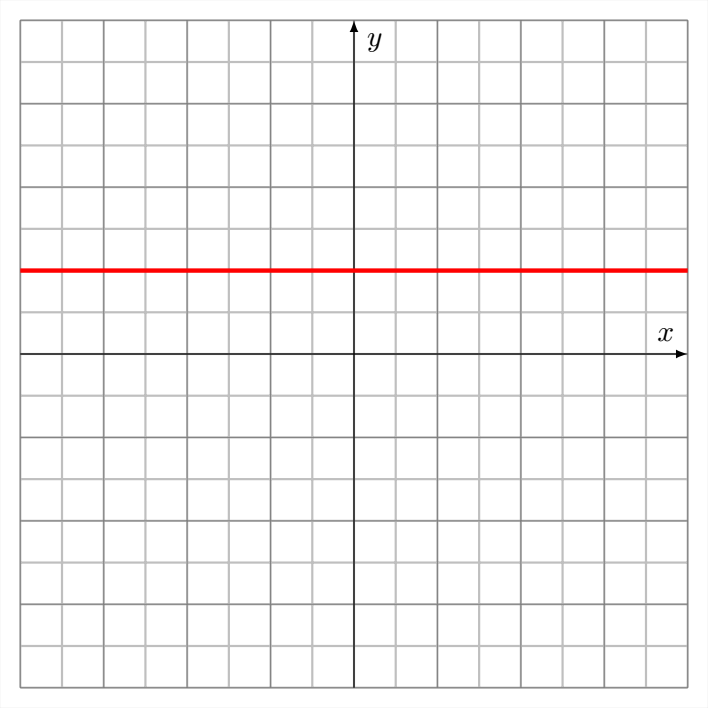
\includegraphics[width=\linewidth]{../images/plano_cart_rect_0.png}
                  \end{minipage}%
                  \begin{minipage}{0.5\linewidth}
                        \begin{choices}
                              \choice Positiva
                              \choice Negativa
                              \CorrectChoice Cero
                              \choice Indefinida
                        \end{choices}
                  \end{minipage}

                  \part
                  \begin{minipage}{0.5\linewidth}
                        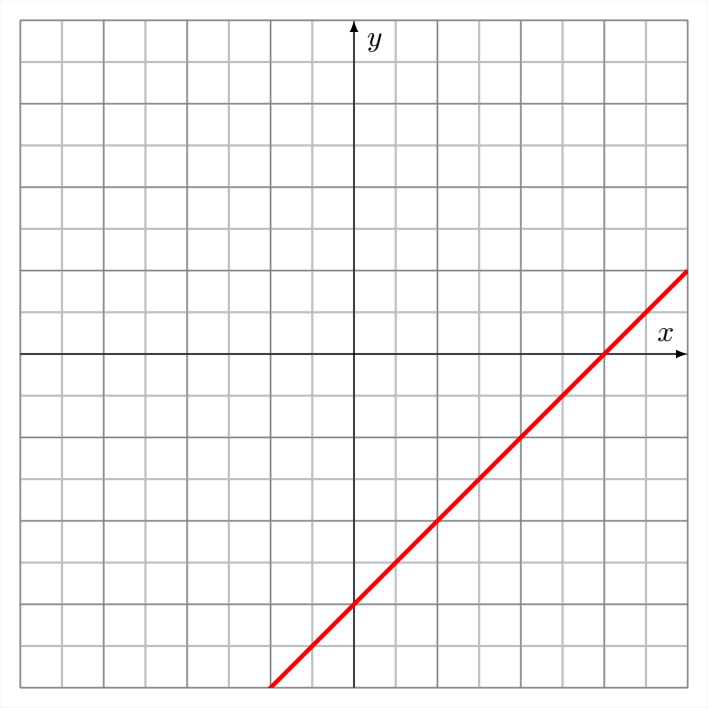
\includegraphics[width=\linewidth]{../images/plano_cart_rect_x-6.png}
                  \end{minipage}%
                  \begin{minipage}{0.5\linewidth}
                        \begin{choices}
                              \CorrectChoice Positiva
                              \choice Negativa
                              \choice Cero
                              \choice Indefinida
                        \end{choices}
                  \end{minipage}

                  \part
                  \begin{minipage}{0.5\linewidth}
                        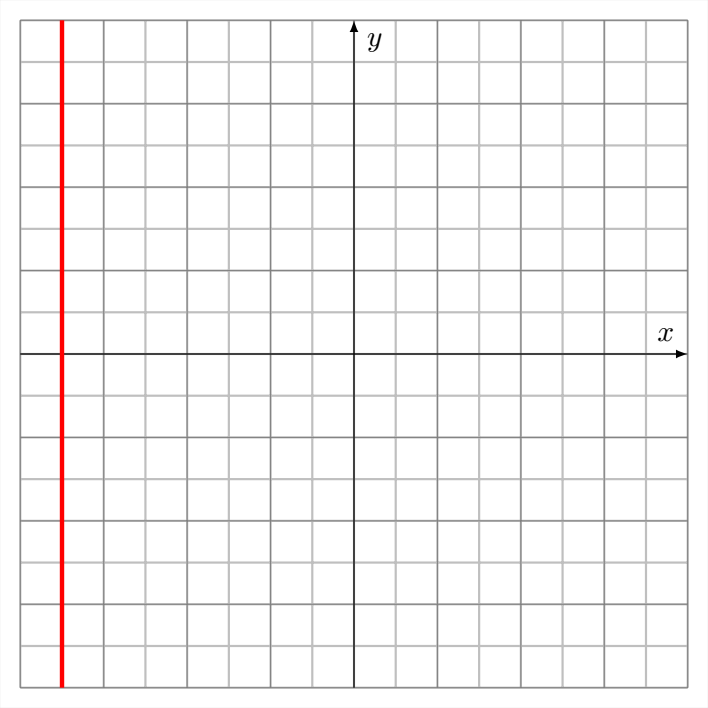
\includegraphics[width=\linewidth]{../images/plano_cart_rect_inf.png}
                  \end{minipage}%
                  \begin{minipage}{0.6\linewidth}
                        \begin{choices}
                              \choice Positiva
                              \choice Negativa
                              \choice Cero
                              \CorrectChoice Indefinida
                        \end{choices}
                  \end{minipage}

                  \part
                  \begin{minipage}{0.5\linewidth}
                        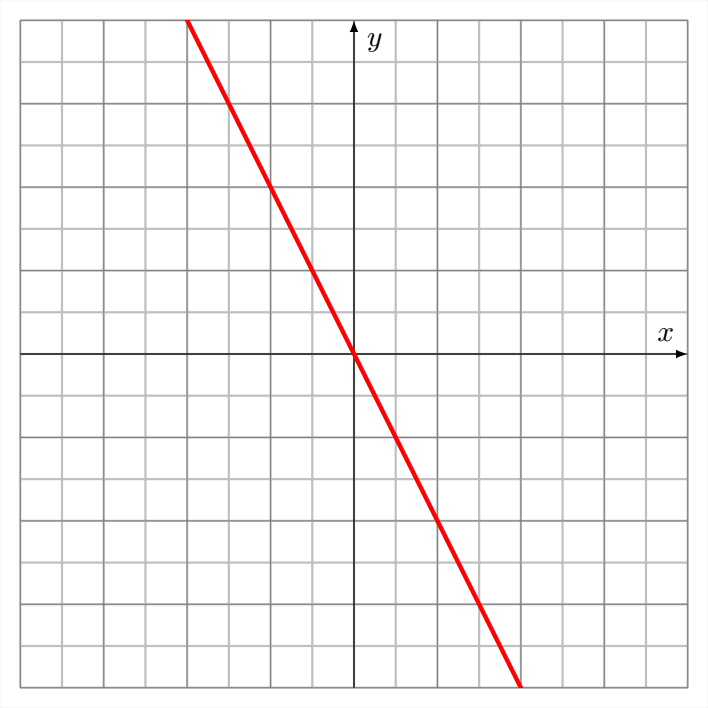
\includegraphics[width=\linewidth]{../images/plano_cart_rect_-2x.png}
                  \end{minipage}%
                  \begin{minipage}{0.5\linewidth}
                        \begin{choices}
                              \choice Positiva
                              \CorrectChoice Negativa
                              \choice Cero
                              \choice Indefinida
                        \end{choices}
                  \end{minipage}
            \end{parts}
      \end{multicols}
      
      \newpage
\addcontentsline{toc}{subsection}{Pendiente y ordenada}
	\subsection*{Pendiente y ordenada}

     
      \question[8] Identifica la pendiente y ordenada de las siguientes rectas:
    
      \begin{multicols}{2}
            \begin{parts}
                  \part  
                  \begin{minipage}{0.4\linewidth}
$y=-2x+1$ 
                  \end{minipage}%
                  \begin{minipage}{0.5\linewidth}
                  Pendiente = \fillin[$-2$][0in]\\[0.5em]
                  Ordenada = \fillin[$1$][0in]
            \end{minipage}

                  \part 
                   \begin{minipage}{0.4\linewidth}
                       $y=-\dfrac{3}{2}x-5$
                                          \end{minipage}%
                                          \begin{minipage}{0.5\linewidth}
                  Pendiente = \fillin[$-\dfrac{3}{2}$][0in]\\[0.5em]
                  Ordenada = \fillin[$-5$][0in]
            \end{minipage}

            \end{parts}
      \end{multicols}


      % \newpage
      
\addcontentsline{toc}{subsection}{Ecuación de una recta}
	\subsection*{Ecuación de una recta}

    
      \question[4] Escribe la \textbf{ecuación} de cada una de las rectas en los siguientes planos cartesianos:
    
      \begin{multicols}{2}
            \begin{parts}
                  \part
                  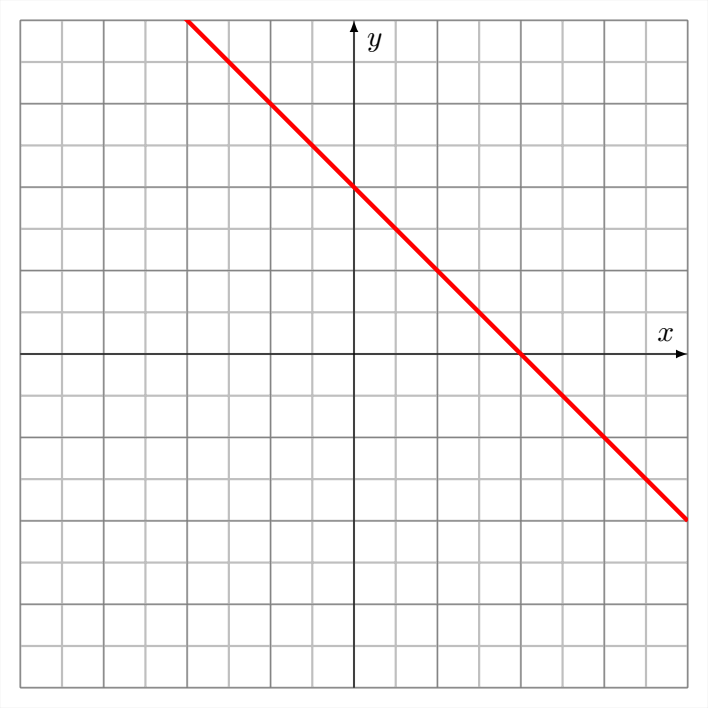
\includegraphics[width=.8\linewidth]{../images/plano_cart_rect_-x+4.png}\\
                  \fillin[$y=-x+4$][2in]

                  \part
                  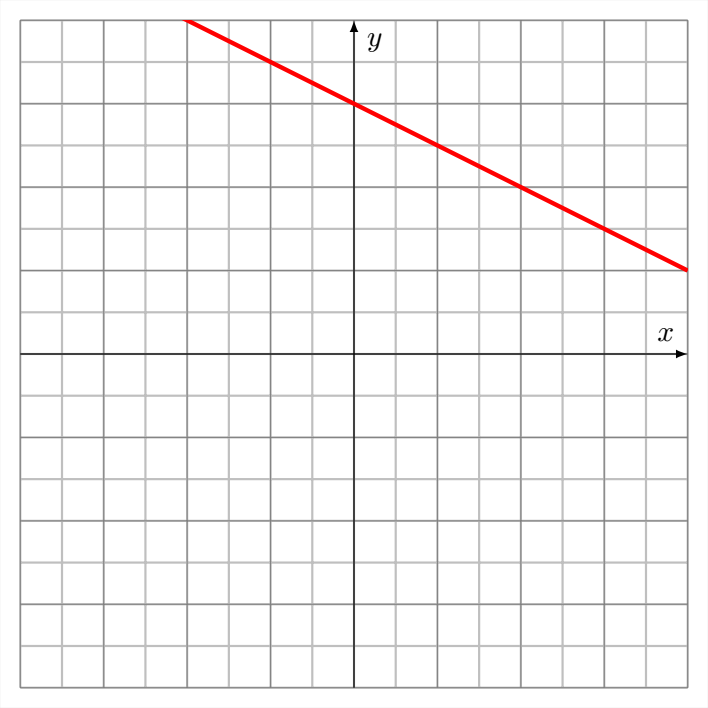
\includegraphics[width=.8\linewidth]{../images/plano_cart_rect_-1|2x+4.png}\\
                  \fillin[$y=-\dfrac{1}{2}x+6$][2in]
            \end{parts}
      \end{multicols}

      \addcontentsline{toc}{section}{Porcentajes}
	\section*{Porcentajes}

      
\addcontentsline{toc}{subsection}{Porcentajes a decimal}
	\subsection*{Porcentajes a decimal}


      \question[4] Escribe el número decimal que representa cada porcentaje:

      \begin{multicols}{2}
            \begin{parts}
                  \part $401\% = \fillin[$0.229$][0in]$
                  \part $6\% = \fillin[$0.062$][0in]$
                  \part $0.5\% =\fillin[$0.005$][0in]$
                  \part $20.9\% = \fillin[$0.209$][0in]$
            \end{parts}
      \end{multicols}

      
\addcontentsline{toc}{subsection}{Decimal a porcentaje}
	\subsection*{Decimal a porcentaje}

      \question[4] Escribe el porcentaje que representa cada número decimal:

      \begin{multicols}{2}
            \begin{parts}
                  \part $0.44  =\fillin[$44\%$][0in]$
                  \part $0.092 =\fillin[$9.2\%$][0in]$
                  \part $5.5  = \fillin[$550\%$][0in]$
                  \part $0.33 = \fillin[$33\%$][0in]$
            \end{parts}
      \end{multicols}

\newpage
      
\addcontentsline{toc}{subsection}{Porcentaje de cantidades}
	\subsection*{Porcentaje de cantidades}

      \question[8] Calcula los porcentajes de cada una de las siguientes cantidades:
   
      \begin{multicols}{2}
            \begin{parts}
                  \part ¿Cuál es el 225\% de 600?
                  
                  \begin{solutionbox}{1.8cm}
                        \[\dfrac{600\times 225\%}{100\%}=1350\]
                  \end{solutionbox}

                  \part Si se sabe que 30 es el 6\% de cierta cantidad, ¿cuál es esta cantidad?
                 
                  \begin{solutionbox}{1.8cm}
                        \[\dfrac{30\times 100\%}{6\%}=500\]
                  \end{solutionbox}

                  \part ¿Cuál es el 23\% de 59?
               
                  \begin{solutionbox}{1.8cm}
                        \[\dfrac{59\times 23\%}{100\%}=13.57\]
                  \end{solutionbox}

                  \part Si se sabe que 40 es el 250\% de cierta cantidad, ¿cuál es esta cantidad?
               
                  \begin{solutionbox}{1.8cm}
                        \[\dfrac{40\times 100\%}{250\%}=16\]
                  \end{solutionbox}
            \end{parts}
      \end{multicols}

      
\addcontentsline{toc}{subsection}{Resolución de problemas}
	\subsection*{Resolución de problemas}

      \question[8] Resuelve los siguientes problemas:
   
      \begin{multicols}{2}
      \begin{parts}
            \part El costo de una camisa es de \$800 pesos, si se les hace un descuento del 20\%, ¿cuánto pagaré en total por la camisa?
            
            \begin{solutionbox}{2cm}
                  \[\$800\times 20\%=\$160\]
                  \[\$800-\$160=\$640\]
            \end{solutionbox}

            \part El 24\% de los habitantes de un pueblo tienen menos de 30 años. ¿Cuántos habitantes tiene el pueblo si hay 120 jóvenes menores de 30 años?
       
            \begin{solutionbox}{2cm}
                  \[\dfrac{120\times 100\%}{24\%}=500\]
            \end{solutionbox}
      \end{parts}
\end{multicols}

\end{questions}
\end{document}